\documentclass[12pt]{beamer}
%\usepackage[spanish]{babel} % Para separar correctamente las palabras
%%\usepackage[utf8]{inputenc} % Este paquete permite poner acentos y eñes usando codificación utf-8
%\usepackage[latin1]{inputenc}

\makeatletter

\usetheme{Antibes}
\usepackage{amssymb}
\usepackage{mathtools}	
\usepackage{amsmath}
\usepackage{dsfont}	
\useoutertheme{infolines}
\usepackage{caption}
\usepackage{subcaption}
\captionsetup{compatibility=false}
\usepackage{amsmath}
\usepackage{algorithm}
\usepackage{algorithmic}


\usetheme{Antibes}
\useoutertheme{infolines}
\title[Deep Reinforcement Learning]{Playing Atari with Deep Reinforcement Learning}
\author[Imanol Arrieta Ibarra]{Volodymyr Mnih, Koray Kavukcuoglu, David Silver, Alex Graves, Ioannis Antonoglou, Daan Wierstra, Martin Riedmiller}

\begin{document}

\begin{frame}
  		\titlepage
\end{frame}

\section{Games}
\begin{frame}
\frametitle{Atari Games}
\centering
			\only<1>{
			\begin{figure} 
			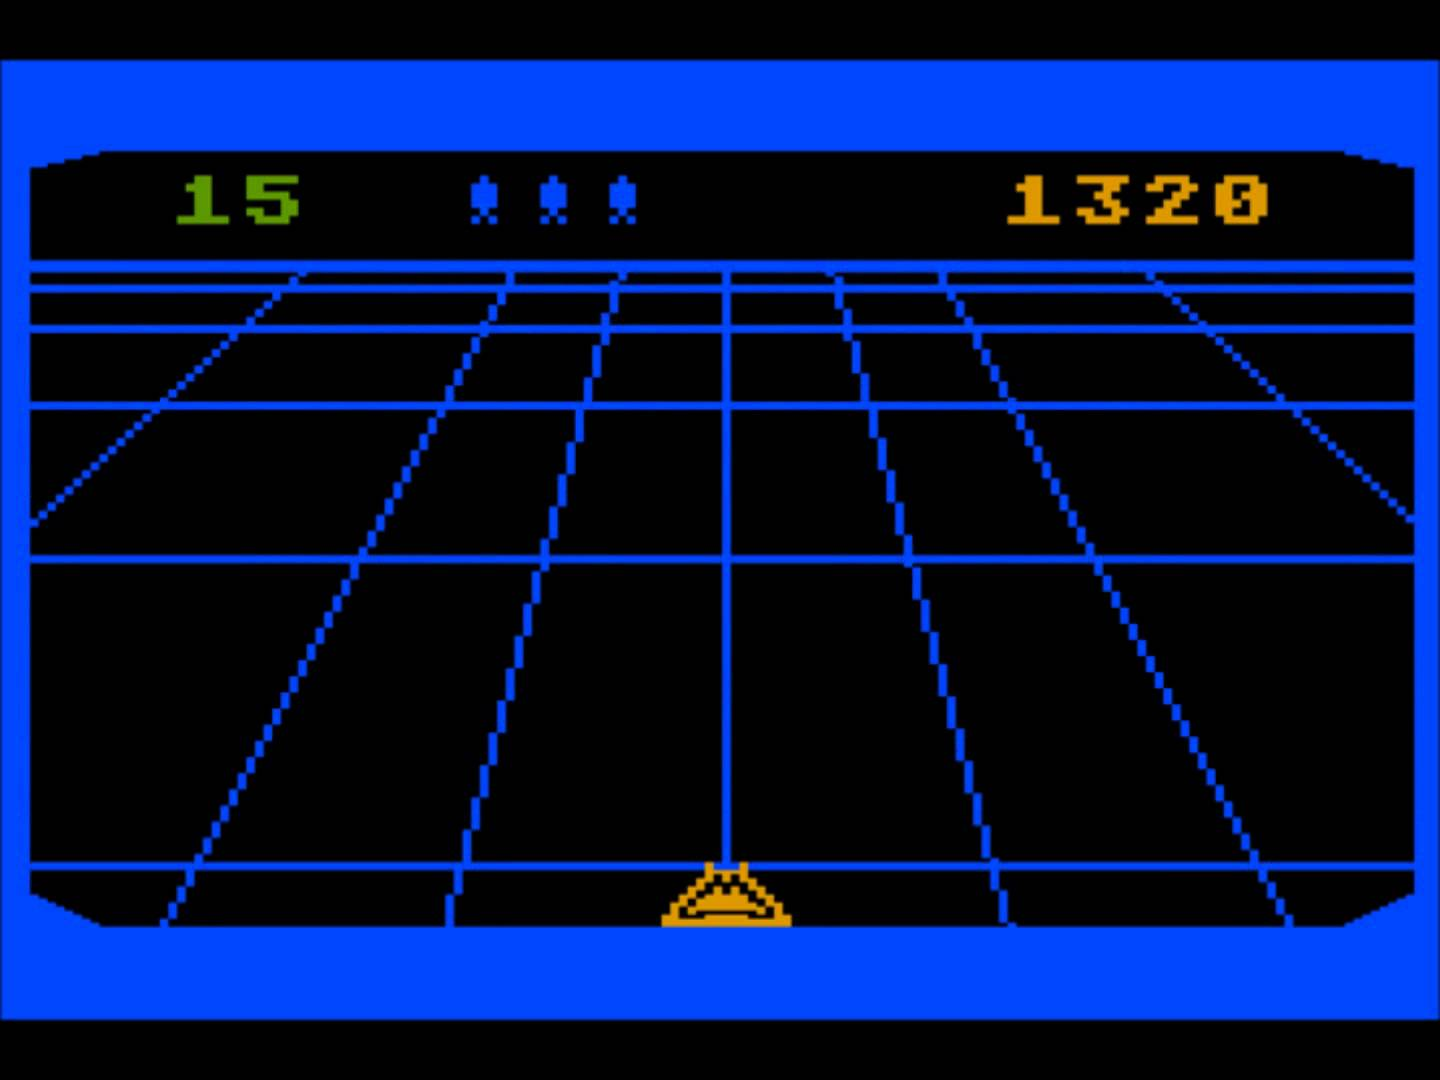
\includegraphics[width = .8\linewidth]{BRider.jpg} 
			\end{figure}
			}
			\pause
			\only<2>{\begin{figure} 
			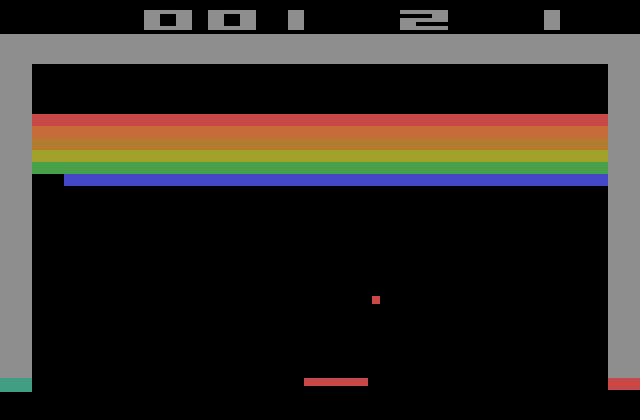
\includegraphics[width = .8\linewidth]{Breakout.png} 
			\end{figure}
			}
			\pause
			\only<3>{\begin{figure} 
			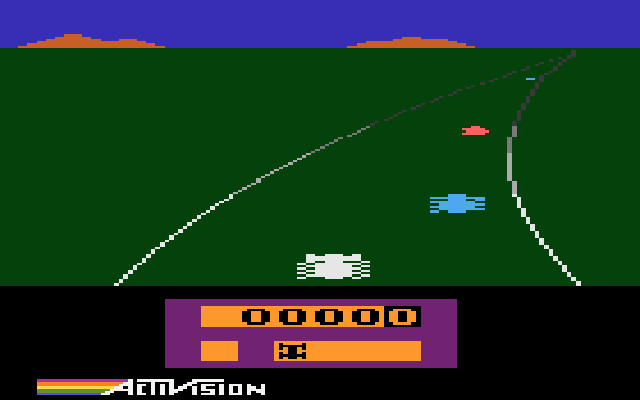
\includegraphics[width = .8\linewidth]{Enduro.png} 
			\end{figure}
			}	
			\pause
			\only<4>{\begin{figure} 
			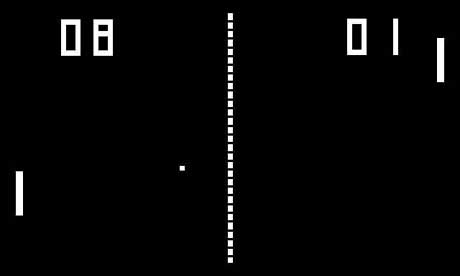
\includegraphics[width = .8\linewidth]{Pong.jpg} 
			\end{figure}
			}	
			\pause
			\only<5>{\begin{figure} 
			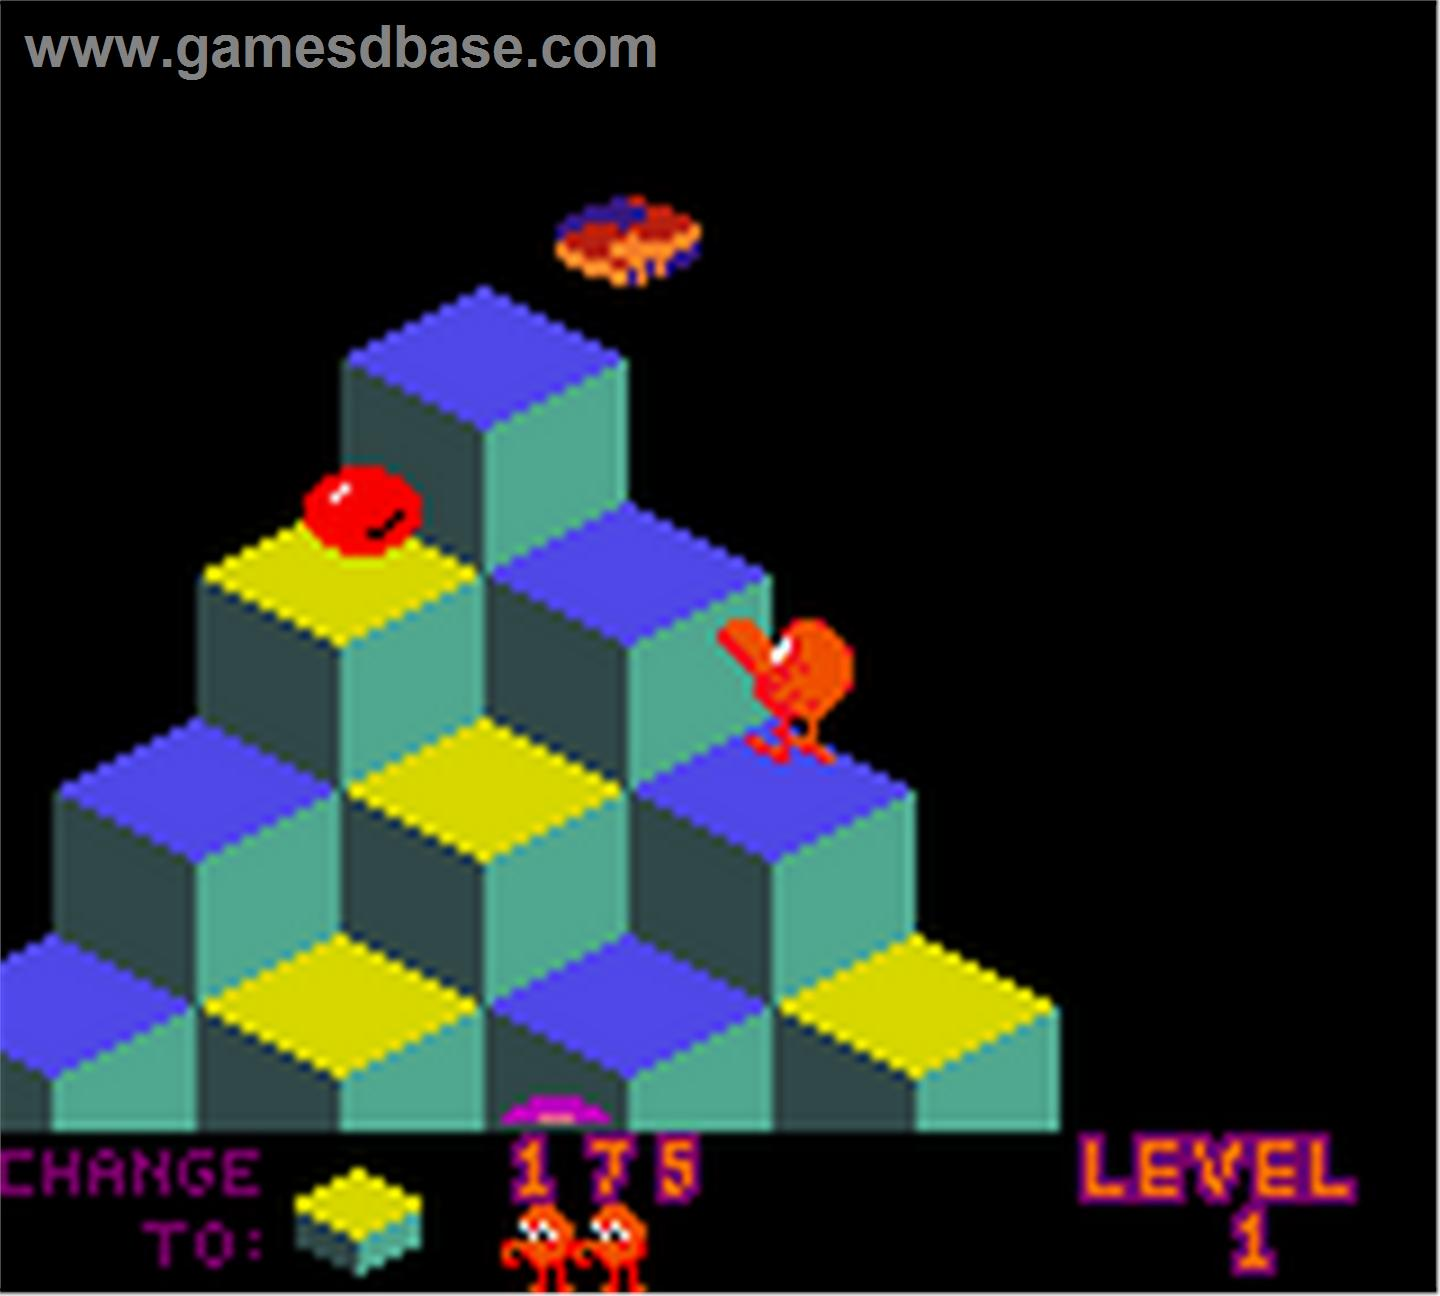
\includegraphics[width = .8\linewidth]{Qbert.jpg} 
			\end{figure}
			}	
			\pause
			\only<6>{\begin{figure} 
			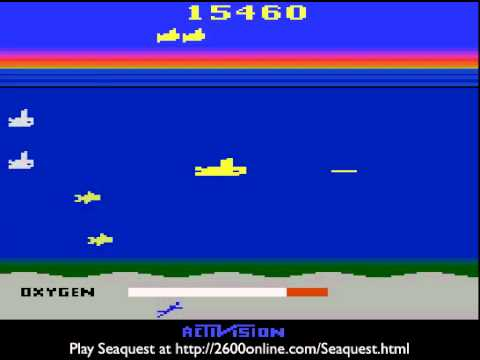
\includegraphics[width = .8\linewidth]{Seaquest.jpg} 
			\end{figure}
			}	
			\pause
			\only<6>{\begin{figure} 
			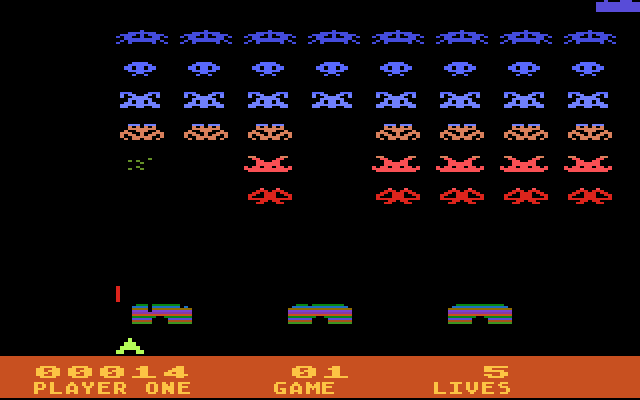
\includegraphics[width = .8\linewidth]{Space.png} 
			\end{figure}
			}						
\end{frame}

\section{Idea}
\begin{frame}
\frametitle{Problem Statement}
\begin{enumerate}
\item Development of a deep learning model that learns to play Atari games.
\item   The only input this model receives is the Atari emulator's output. 
\item They use convolutional neural networks trained with a variant of Q-learning whose input is raw pixels and output is a value function estimating future rewards.
\end{enumerate}

\end{frame}

\section{Model Setup}

\begin{frame}
\frametitle{The Model}
\centering
			\only<1>{
			\begin{figure} 
			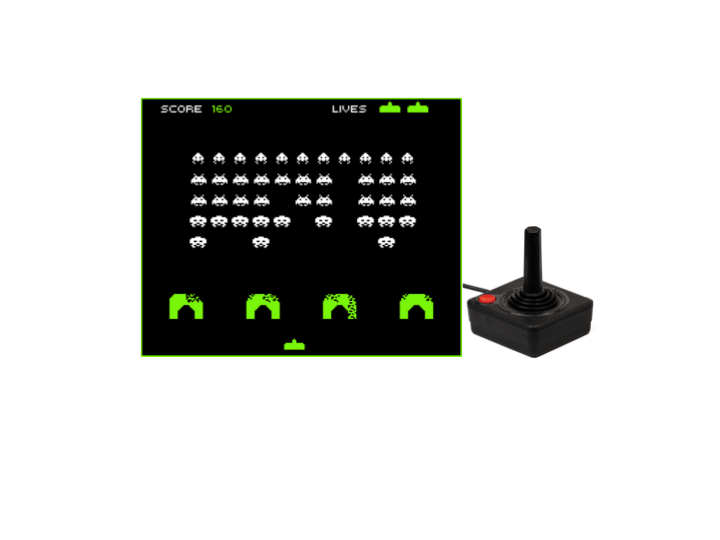
\includegraphics[width = .8\linewidth]{Slide1.png} 
			\end{figure}
			}
			\pause
			\only<2>{\begin{figure} 
			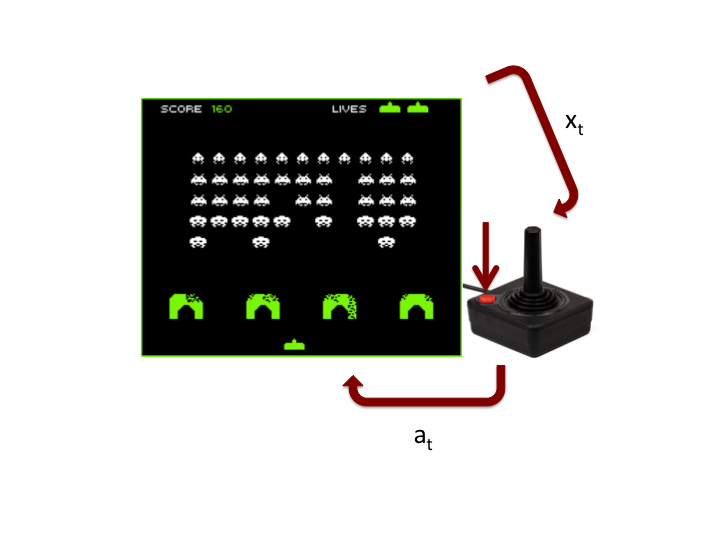
\includegraphics[width = .8\linewidth]{Slide2.png} 
			\end{figure}
			}
			\pause
			\only<3>{\begin{figure} 
			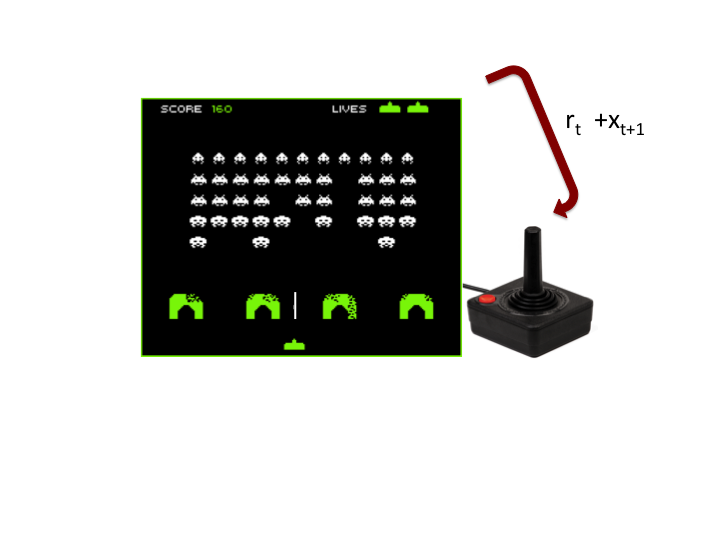
\includegraphics[width = .8\linewidth]{Slide3.png} 
			\end{figure}
			}						
\end{frame}

\begin{frame}
\frametitle{Sequence of states}
\begin{itemize}
\item It is difficult to make sense of the visual input from only one frame. So the learning algorithm will take a sequence of images and actions as the state.
\item $s_t=x_1,a_1,x_2,a_2,...,a_{t-1},x_t$
\item They define the future discounted return at time t as: $$R_t = \sum\limits_{t'=t}^T\gamma^{t'-t}r_{t'}$$
\item They define the optimal action-value function:
$$Q*(s,a) = max_{\pi}\mathbb{E}[R_t|s_t=s,a_t=a,\pi]$$
\end{itemize}
\end{frame}


\begin{frame}
\frametitle{Bellman Equation and Function Approximation}
\begin{itemize}
\item The Bellman equation is defined as:
$$Q*(s,a) = \mathbb{E}_{s'\sim \xi}[r+\gamma max_{a'}Q*(s',a')|s,a]$$
\item We would like to approximate $Q*(s,a)\approx Q(s,a;\theta)$
\item We can use a neural network and fit it to the data by minimizing at each iteration:$$L_i(\theta_i) = \mathbb{E}_{s,a \sim \rho(\cdot)}[(y_i-Q(s,a;\theta_i))^2]$$
$$y_i = \mathbb{E}_{s'\sim \xi} [r+\gamma max_{a'}Q(s',a';\theta_{i-1})|s,a]$$
\end{itemize}
\end{frame}

\begin{frame}
\frametitle{Model fitting}
\begin{enumerate}
\item The gradient of the loss function is:
\begin{scriptsize}
$$\nabla_{\theta_i}L_i(\theta_i) = \mathbb{E}_{s,a\sim \rho(\cdot);s'\sim \xi} \left[\left(r+\gamma max_{a'}Q(s',a';\theta_{i-1}) - Q(s,a;\theta_i)\right)\nabla_{\theta_i}Q(s,a;\theta_i)\right]$$
\end{scriptsize}
\item We can instead compute Stochastic Gradient Descent
\item Instead of computing the expectation we only sample from the distribution of future states, we get Q-learning.
\end{enumerate}
\end{frame}

\section{Preprocessing}
\begin{frame}
\frametitle{Preprocessing}
\begin{itemize}
\item Atari frames are 210x160 pixel images in 128 color palette. So for each $x_t$ image, they define a preprocessing stage where they turn images into a gray-scale, down-sampling the image to a 110x84 image. Then they crop the image down to a 84x84 region.
\item Given a sequence of images and actions : $s_t = x_1,a_1,...a_{t-1},x_{t}$ they define $\phi(s_t)$ as only considering the last four frames and processing the corresponding images.
\item For the neural network, they use an architecture in which there is a separate output unit for each action, and the state representation is the only input.
\end{itemize}
\end{frame}

\section{Algorithm}
\begin{frame}
\frametitle{Deep Q-Learning with Experience Replay}
\begin{algorithm}[H]
\begin{algorithmic}[1]
\scriptsize
\STATE Initialize replay memory $\mathcal{D}$ to capacity N.
\STATE Initialize action-value function $\mathcal{Q}$ with random weights.
\FOR{$episode=1$ to $M$}
\STATE Initialize sequence $s_1 = \{x_1\}$ and preprocess $\phi_1 = \phi(s_1)$.
\FOR{$t=1$ to $T$}
\STATE With probability $\epsilon$ select a random action $a_t$.
\STATE Execute action $a_t$ in emulator and observe reward $r_t$ and image $x_{t+1}$ 
\STATE Set $s_{t+1} = s_t, a_t, x_{t+1}$ and preprocess $\phi_{t+1} = \phi(s_{t+1})$.
\STATE Store transition $(\phi_t, a_t,r_t,\phi_{t+1})$ in $\mathcal{D}$.
\STATE Sample random minibatch of transitions $(\phi_j,a_j,r_j,\phi_{j+1})$ from $\mathcal{D}$.
\STATE Set \begin{displaymath}
   y_j = \left\{
     \begin{array}{lr}
       r_j & : \text{for terminal }\phi_{j+1}\\
       r_j + \gamma max_{a'} \mathcal{Q}(\phi_{j+1},a';\theta) & : \text{o.w.}
     \end{array}
   \right.
\end{displaymath} 
\STATE Perform a gradient descent step on $(y_j-\mathcal{Q}(\phi_j,a_j;\theta))^2$
\ENDFOR
\ENDFOR
\end{algorithmic}
\caption{Deep Q-Learning with Experience Replay}
\label{alg:seq}
\end{algorithm}
\end{frame}

\section{Convolutional Neural Network}
\begin{frame}
\frametitle{Architecture}
\begin{figure}[h]
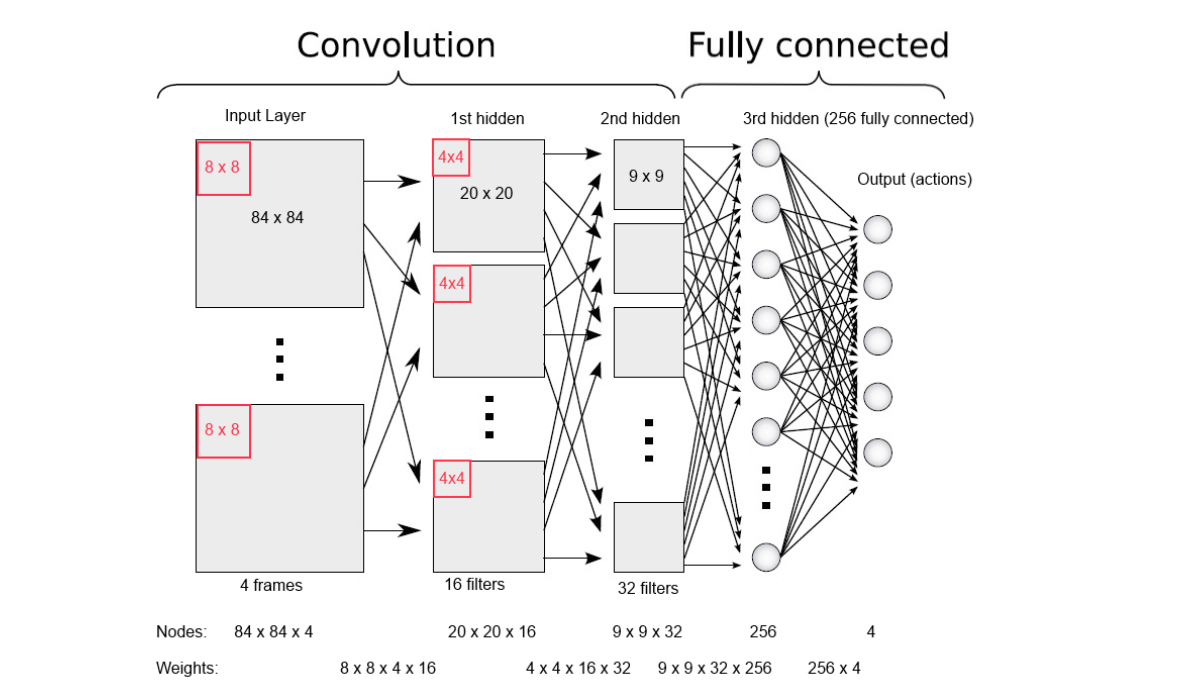
\includegraphics[scale=.3]{NN.png}
\end{figure}
\end{frame}

\section{Results}
\begin{frame}
\frametitle{Value Function}
\begin{figure}[h]
\centering
\includegraphics[scale=.3]{sub.png}
\end{figure}
\end{frame}

\begin{frame}
\frametitle{Comparison with previous algorithms and human players}
\begin{figure}[h]
\centering
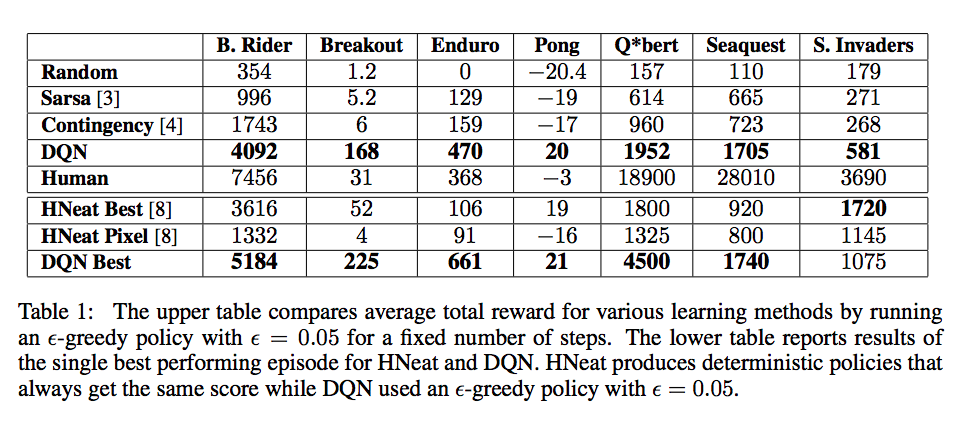
\includegraphics[scale=.35]{Results.png}
\end{figure}
\end{frame}

\section{Key Insights}
\begin{frame}
\frametitle{Epsilon Greedy}
\begin{itemize}
\item Using epsilon-greedy may not be an issue for the absence of really delayed consequences.
\item In general only optimizing for close time frames may be sufficient to optimize rewards.
\end{itemize}
\end{frame}

\begin{frame}
\frametitle{Replay Memory}
\begin{itemize}
\item For neural networks and other supervised learning algorithms it is important for the samples to be independent. 
\item By sampling from previous runs of the algorithm, they are able to break the correlation between states.
\end{itemize}
\end{frame}


%\section{Crisis de Violencia}
%\subsection{Datos Hist\'oricos}
%\begin{frame}
%\frametitle{La Guerra contra el Narcotr\'afico}
%\begin{itemize}
%	\item A principios de 2007, el gobierno de Felipe Calder\'on Hinojosa declar\'o la guerra al crimen organizado.
%	\item M\'as de 200 municipios han sido afectados.
%	\item 64000 personas han muerto como consecuencia de esta guerra.
%	\item El n\'umero de ejecuciones, secuestros y extorsiones ha aumentado desproporcionadamente desde ese momento.
%\end{itemize}
%\end{frame}
%
%\begin{frame}
%\frametitle{Estados con m\'as de 35 muertes al mes}
%\centering
%			\only<1>{
%			\begin{figure} 
%			\includegraphics[width = .8\linewidth]{Diciembre2006.pdf} 
%			\caption{Diciembre 2006}
%			\end{figure}
%			}
%			\pause
%			\only<2>{\begin{figure} 
%			\includegraphics[width = .8\linewidth]{Diciembre2007.pdf} 
%			\caption{Diciembre 2007}
%			\end{figure}
%			}
%			\pause
%			\only<3>{\begin{figure} 
%			\includegraphics[width = .8\linewidth]{Diciembre2008.pdf} 
%			\caption{Diciembre 2008}
%			\end{figure}
%			}
%			\pause
%			\only<4>{\begin{figure} 
%			\includegraphics[width = .8\linewidth]{Diciembre2009.pdf} 
%			\caption{Diciembre 2009}
%			\end{figure}
%			}
%			\pause
%			\only<5>{\begin{figure} 
%			\includegraphics[width = .8\linewidth]{Diciembre2010.pdf} 
%			\caption{Diciembre 2010}
%			\end{figure}
%			}
%			
%\end{frame}
%
%\begin{frame}
%\frametitle{Evoluci\'on de la Violencia}
%\includegraphics[width = \linewidth]{Homicidios_SEGOB.pdf}
%\end{frame}
%
%\begin{frame}
%\frametitle{Violencia en los Estados}
%\only<1>{ \begin{figure}
%\caption{N\'umero de Ejecuciones en Chihuahua}
%\centering
%\includegraphics[width = .8\linewidth]{ChihuahuaEdo.pdf}
%\end{figure}}
%			\pause
%			\only<2>{\begin{figure}
%		\caption{N\'umero de Ejecuciones en Coahuila}
%\includegraphics[width = .8\linewidth]{Coahuila.pdf}
%\end{figure}}
%			\pause
%			\only<3>{\begin{figure}
%			\caption{N\'umero de Ejecuciones en Durango}
%\includegraphics[width = .8\linewidth]{Durango.pdf}
%\end{figure}}
%			\pause
%			\only<4>{\begin{figure}
%	\caption{N\'umero de Ejecuciones en el Estado de M\'exico}
%\includegraphics[width = .8\linewidth]{Mexico.pdf}
%\end{figure}}
%			\pause
%			\only<5>{\begin{figure}
%\caption{N\'umero de Ejecuciones en Tamaulipas}
%\includegraphics[width = .8\linewidth]{Tamaulipas.pdf}
%\end{figure}}
%			\pause
%			\only<6>{\begin{figure}
%			\caption{N\'umero de Ejecuciones en Jalisco}
%\includegraphics[width = .8\linewidth]{Jalisco.pdf}
%\end{figure}}
%			\pause
%			\only<7>{\begin{figure}
%			\caption{N\'umero de Ejecuciones en Nuevo Le\'on}
%\includegraphics[width = .8\linewidth]{NuevoLeon.pdf}
%\end{figure}}
%\end{frame}
%
%\section{Costo Econ\'omico de la Crisis de Violencia}
%\subsection{Indice Trimestral de Actividad Econ\'omica Estatal}
%
%\begin{frame}
%\begin{itemize}
%	\item El punto de esta investigaci\'on es el cuantificar el efecto de la crisis de violencia en la actividad econ\'omica mexicana.
%	\item Se usa el ITAEE, cuyo calculo sigue las mismas reglas que el PIB.
%	\item ?`C\'omo se habr\'ia desempe\~nado M\'exico de no haber existido la crisis de violencia?
%\end{itemize}
%\end{frame}
%
%\section{Controles Sint\'eticos para Estudios de Casos Comparativos}
%\subsection{Explicaci\'on}
%\begin{frame}
%
%\begin{figure}[h]
%\caption{Efectos del Narcotr\'afico en M\'exico}
%	\centering
%	\begin{subfigure}[b]{.45\textwidth}
%		\centering
%		\includegraphics[width=\textwidth]{Bandera1.jpg}
%		\caption{M\'exico con Narcotr\'afico}
%	\end{subfigure}
%	\begin{subfigure}[b]{.45\textwidth}
%		\centering
%		\includegraphics[width=\textwidth]{Bandera2.jpg}
%		\caption{M\'exico sin Narcotr\'afico}
%	\end{subfigure}
%	\label{gr:CiudadJuarez_Chi}
%	\end{figure}
%	
%\end{frame}
%
%\subsection{Caso Univariado}
%\begin{frame}
%
%\frametitle{Variables}
%
%	Sean
%	 \vspace{0.2cm}
% 
%	\begin{itemize}
%		\item  $J+1$ regiones, 1 regi\'on de tratamiento y $J$ regiones de control (15 regiones, Chihuahua y 14 regiones de control) \pause
%		\item $T_0$ es el n\'umero de periodos previos al tratamiento donde $0 \leq  T_{0}  \leq T$. Para el ITAEE tenemos $T_0=22$ y $T=40$
%		\item $Y_{it}^N$ la observaci\'on de la regi\'on $i$ en el tiempo $t$ sin tratamiento $t \in \{1, \dots, T_{0}\}$. Por ejemplo, $Y_{Chihuahua2006}^{N}$  o $Y_{Chiapas2007}^{N}$\pause
%		\item $Y_{it}^I$ la observaci\'on de la regi\'on $i$ en el tiempo $t$ con tratamiento $t \in \{T_{0+1}, \dots, T\}$. Por ejemplo, $Y_{Chihuahua2008}^I$ \pause
%	\end {itemize} 
%
%	\vspace{0.2cm}
%
%	Por lo que se tiene $Y_{it}^I$= $Y_{it}^N$ para $t \in \{1, \dots, T_{0}\}$ \pause
%	\vspace{0.2cm}
%
%	Se asume que las regiones de control no son afectadas con el inicio del tratamiento. \\
%
%\end{frame}
%
%
%
%
%\begin{frame}
%\frametitle{Objetivo del modelo}
%
%	\begin{itemize}
%		\item Definimos el efecto del tratamiento sobre la regi\'on $i$ como 
%		$$\alpha_{it} = Y_{it}^I-Y_{it}^N$$
%		$$\alpha_{Chihuahua2008} = Y_{Chihuahua2008}^I-Y_{Chihuahua2008}^N$$ \pause
%		\item El objetivo es estimar $\alpha_{it}$ para $t>T_{0}$ $(t>2008)$\pause \\
%		\item Nosotros conocemos $Y_{it}^I$, por lo que nos faltar\'ia estimar $Y_{it}^N$. \pause
%		\vspace{0.2cm}		
%		Supongamos que $Y_{it}^N$ es representado por el siguiente modelo: \\
%
%		$$Y_{it}^N = \delta_{t} + \theta_{t} \mathds{Z}_{i} + \lambda_{t} \mu_{i} + \varepsilon_{it}$$ \pause
%		Donde
%		\item $\delta_{t}$ un factor com\'un desconocido \pause
%		\item $\mathds{Z}_{i}$ un vector de $r x 1$ de variables observadas no afectadas por el tratamiento (caracter\'isticas o predictores utilizados)
%
%		\vspace{0.2cm}
%
%	\end{itemize}
%
%\end{frame}
%
%
%
%\begin{frame}
%	\frametitle{Par\'ametros del modelo}
%	\begin{itemize}
%
%		\item $\lambda_{t}$ un vector de factores com\'unes no observables (cultura) \pause
%		\item $\mu_{i}$ un vector de pesos desconocido \pause
%		\item $\varepsilon_{it}$ shocks transitorios no observables con media cero \pause
%		\item Sea $\mathds{W}$ un vector de pesos $\mathds{W} = (w_{2}, ... , w_{J+1})'$ de dimensi\'on $J x 1$ \\
%		$$w_{j}  \geq 0 \text{ y } j=2,..., J+1$$
%		$$w_{2}+w_{3}+...+w_{J+1} = 1$$ \pause
%
%		\item Para cada vector de pesos $\mathds{W}$  se obtiene un control sint\'etico diferente, el cual es una combinaci\'on lineal (promedio ponderado) de las regiones de control 
%
%	\end{itemize}
%
%\end{frame}
%
%
%\begin{frame}
%	\frametitle{Controles Sint\'eticos}
%
%	Supongamos existen $(w_{2}{*}, ... , w_{J+1}{*})'$ tales que
%	$$\sum_{j=2}^{J+1}w_{j}^{*}Y_{j1} = Y_{11}$$
%	$$\sum_{j=2}^{J+1}w_{j}^{*}Y_{j2} = Y_{12}$$
%	$$ ... $$
%	$$\sum_{j=2}^{J+1}w_{j}^{*}Y_{jT_{0}} = Y_{1T_{0}}$$
%	$$\sum_{j=2}^{J+1}w_{j}^{*}Z_{j} = Z_{1}$$ \pause
%	
%
%\end{frame}
%
%\begin{frame}
%\frametitle{Identificaci\'on del Efecto}
%
%
%	$$\Rightarrow \alpha_{it} = Y_{1t} - \sum_{j=2}^{J+1}w_{j}^{*}Y_{t} \text{ para } t \in \{T_{0+1}, \dots, T\}$$ \\ \pause
%	Para que se cumpla esto, se necesita que $(Y_{11},Y_{12},...,Y_{1T_{0}}, Z_{1}^{'})$ pertenezca al espacio convexo de  {$(Y_{21},Y_{22},...,Y_{2T_{0}}, Z_{2}^{'}), ... , (Y_{J+1 1},Y_{J+1 2},...,Y_{J+1 T_{0}}, Z_{J+1}^{'})$}
%
%
%\end{frame}
%
%
%\section{Splines C\'ubicos para expandir la base de predictores}
%\subsection{Motivaci\'on}
%\begin{frame}
%\frametitle{Proceso Generador de Datos}
%\begin{itemize}
%\item Con el fin de mejorar el sesgo de las estimaciones podemos relajar el supuesto de linealidad en los predictores del proceso generador de datos a:
%$$Y_{it}^N = \delta_{t} + \theta_{t} f(\mathds{Z}_{i}) + \lambda_{t} \mu_{i} + \varepsilon_{it}$$ \pause
%\item Para limitar el n\'umero de posibles funciones supondr\'e que: 
% $$f: \mathbb{R}^r \rightarrow \mathbb{R}$$
% $$f(\boldsymbol{Z}_i;\theta_t) = \sum\limits_{l=1}^r \theta_{tl}f_l(\boldsymbol{Z}_{il})$$
% $$ f_l:[\psi_{l1},\psi_{l2}] \rightarrow [\psi_{l3},\psi_{l4}]$$
%\end{itemize}
%\end{frame}
%
%\begin{frame}
%\frametitle{Sesgo Asint\'otico}
%\begin{itemize}
%\item En el Ap\'endice A de mi tesis demuestro que :
% $$\mathbb{E}[\hat{\alpha}_{1t}]=\boldsymbol{\lambda}_t (\boldsymbol{\lambda}^{P'} \boldsymbol{\lambda}^{P})^{-1} \boldsymbol{\lambda}^{P'}\left(f(\boldsymbol{Z_{1}};\theta_t)- \sum\limits_{j=2}^{J+1}w_j f(\boldsymbol{Z}_{j};\theta_t)\right) \neq 0.$$
%\end{itemize}
%\end{frame}
%
%\begin{frame}
%\frametitle{Aproximaci\'on por Splines}
%Usando splines c\'ubicos con $K$ nudos, se pedir\'ia a los controles sint\'eticos satisfacer:
%\begin{equation}
%\label{eq:Cont_Syn_Im}
%h_{il}(\boldsymbol{Z}_{1l})= \sum\limits_{j=2}^{J+1}h_{il}(\boldsymbol{Z}_{jl}),\quad  \forall i= 1,...,K, \quad \forall l=1,...,r
%\end{equation}
%\end{frame}
%
%\begin{frame}
%\frametitle{Soluci\'on del sesgo}
%\footnotesize
%\begin{equation}
%\begin{array}{ccl}
%\mathbb{E}[\hat{\alpha}_{1t}]&=&\boldsymbol{\lambda}_t (\boldsymbol{\lambda}^{P'} \boldsymbol{\lambda}^{P})^{-1} \boldsymbol{\lambda}^{P'}\left(f(\boldsymbol{Z_{1}})- \sum\limits_{j=2}^{J+1}w_j f(\boldsymbol{Z}_{j};\theta_t)\right) \\
%&=&\boldsymbol{\lambda}_t (\boldsymbol{\lambda}^{P'} \boldsymbol{\lambda}^{P})^{-1} \boldsymbol{\lambda}^{P'}\left(f(\boldsymbol{Z_{1}})- h(\boldsymbol{Z_{1}}) + \sum\limits_{j=2}^{J+1}w_j\*h(\boldsymbol{Z_{j}})- \sum\limits_{j=2}^{J+1}w_j f(\boldsymbol{Z}_{j};\theta_t)\right) \\
%&=&\boldsymbol{\lambda}_t (\boldsymbol{\lambda}^{P'} \boldsymbol{\lambda}^{P})^{-1} \boldsymbol{\lambda}^{P'}\left(f(\boldsymbol{Z_{1}})- h(\boldsymbol{Z_{1}}) + \sum\limits_{j=2}^{J+1}w_j\*(h(\boldsymbol{Z_{j}})- f(\boldsymbol{Z}_{j};\theta_t))\right).
%\end{array}
%\end{equation}
%\end{frame}
%
%\section{Splines C\'ubicos para predecir la variable de inter\'es}
%\subsection{Motivaci\'on}
%
%
%\begin{frame}
%\frametitle{Predicci\'on de $Y_{it}^N$}
%\begin{itemize}
%\item Otra forma de analizar Controles Sint\'eticos es como un modelo de predicci\'on donde:
%$$\hat{Y^{N}_{1t}} = f(Y_{2,t},...,Y_{J+1,t};\boldsymbol{\theta}).$$
%\item Con la expansi\'on de base, un control sint\'etico generalizado ser\'ia un vector de pesos $\boldsymbol{\Theta}$ de dimensi\'on ($\sum\limits_{j=1}^{J+1} N_j \times 1$) y una funci\'on $f(Y;\Theta)= \sum\limits_{j=1}^{J+1} \sum\limits_{i=1}^{N_j} \theta_{j,i}h_{j,i}(Y_j)$.
%\end{itemize}
%\end{frame}
%
%\subsection{Hsiao, Ching y Wan}
%\begin{frame}
%\frametitle{Proceso Generador de Datos}
%\begin{equation}
%Y_{it} = \underline{b}_i' \underline{f}_t + \alpha_i +\epsilon_{it}.
%\end{equation}
%Donde $\underline{f}_t$ representa una serie de caracter\'isticas compartidas entre distintas regiones, $\underline{b}_i$ es un vector de pesos de dichas caracter\'isticas para cada regi\'on, $\alpha_i$ son factores intr\'insecos de la regi\'on, y $\epsilon_{it}$ es un t\'ermino de error con media cero y varianza conocida.
%\end{frame}
%
%\begin{frame}
%\frametitle{Modelo}
%\begin{itemize}
%\item Hsiao et al. proponen estimar el efecto del tratamiento como:
%\begin{equation}
%Y_{1t}-\sum\limits_{j=2}^{J+1} b_j^*Y_{jt}.
%\end{equation}
%\item Usando expansi\'on de Splines, se puede estimar el efecto del tratamiento como:
%\begin{equation}
%\hat{\alpha}_{1t} = Y_{1t} - \sum\limits_{j=2}^{J+1} \sum\limits_{i=1}^N b_{ji}^*\*h_{ji}(Y_{jt}). 
%\end{equation}
%
%\end{itemize}
%\end{frame}
%
%\begin{frame}
%\frametitle{Penalizaci\'on}
%\footnotesize
%Para corregir la varianza  de los coeficientes y poder resolver el problema de minimizaci\'on:
%\begin{equation}
%\begin{array}{cc}
%\underset{\lambda}{\text{min}}&CV(\lambda) = \frac{1}{T_0}\sum\limits_{t=1}^{T_0} \left[ Y_{1t}-\hat{\beta}_0(-\kappa(t)) - \sum\limits_{j=2}^{J+1}\sum\limits_{k=1}^{K+4} h_{jk}(Y_{jt})\hat{\beta}_{jk}(-\kappa(t),\lambda)\right]^2,
%\end{array}
%\end{equation}
%
%\begin{equation}
%\begin{array}{cc}
%\hat{\beta}(-\kappa(t),\lambda) & = \underset{\beta}{argmin} \left\lbrace \sum\limits_{\tau \neq t}(T_{i \tau}-\hat{\beta}_0 - \sum\limits_{j=1}^p \sum\limits_{k=1}^{K+4} h_{jk}(Y_{jt})\beta_{jk})^2 + \lambda\sum\limits_{j=1}^p|\beta_{jk}| \right\rbrace.
%\end{array}
%\end{equation}
%\end{frame}
%
%
%\section{Resultados}
%\subsection{Controles Sint\'eticos}
%
%\begin{frame}
%\frametitle{Efecto sobre Chihuahua}
%\begin{figure}[h]
%	\centering
%	\begin{subfigure}[b]{.45\textwidth}
%		\centering
%		\includegraphics[trim=2cm 8cm 3cm 8cm,clip=true,scale=.35]{Chihuahua_Sintetico.pdf}
%		\caption{Control Sint\'etico}
%	\end{subfigure}
%	\begin{subfigure}[b]{.45\textwidth}
%		\centering
%		\includegraphics[trim=2cm 8cm 3cm 8cm,clip=true,scale=.35]{Efecto_Placebo_Chihuahua.pdf}
%		\caption{Efecto Placebo}
%	\end{subfigure}
%	\caption{Efectos en Chihuahua}
%	\label{gr:CS_Chihuahua}
%	\end{figure}
%\end{frame}
%
%
%\begin{frame}
%\frametitle{Efecto sobre Tamaulipas}
%\begin{figure}[!h]
%	\centering
%	\begin{subfigure}[b]{.45\textwidth}
%		\centering
%		\includegraphics[trim=2cm 8cm 3cm 8cm,clip=true,scale=.35]{Tamaulipas_Sintetico.pdf}
%		\caption{Control Sint\'etico}
%	\end{subfigure}
%	\begin{subfigure}[b]{.45\textwidth}
%		\centering
%		\includegraphics[trim=2cm 8cm 3cm 8cm,clip=true,scale=.35]{Efecto_Placebo_Tamaulipas.pdf}
%		\caption{Efecto Placebo}
%	\end{subfigure}
%	\caption{Efectos en Tamaulipas}
%	\label{gr:CS_Tamaulipas}
%	\end{figure}
%\end{frame}
%
%\begin{frame}
%\frametitle{Efecto Promedio de la Violencia en los Estados}
%\begin{table}[!ht]
%\centering 
%\begin{tabular}{ccccc}
%\hline \hline
%Tiempo & Efecto & Valor p & Efecto Relativo & Valor p Relativo\\
% 1 &  -0.177 & 0.0000 & -0.001 & 0.0000 \\ 
% 2 &  -1.305 & 0.0000 & -0.010 & 0.0000 \\ 
% 3 &  -1.891 & 0.0000 & -0.015 & 0.0000 \\ 
% 4 &  -1.392 & 0.0000 & -0.011 & 0.0000 \\ 
% 5 &  -2.360 & 0.0000 & -0.020 & 0.0000 \\ 
% 6 &  -1.660 & 0.0000 & -0.013 & 0.0000 \\ 
% 7 &  -2.875 & 0.0000 & -0.023 & 0.0000 \\ 
% 8 &  -2.433 & 0.0000 & -0.020 & 0.0000 \\ 
% 9 &  -3.020 & 0.0000 & -0.023 & 0.0000 \\ 
%10 &  -2.398 & 0.0000 & -0.018 & 0.0000 \\ 
%11 &  -2.636 & 0.0000 & -0.019 & 0.0000 \\ 
%12 &  -2.911 & 0.0000 & -0.022 & 0.0000 \\ 
%13 &  -2.845 & 0.0000 & -0.021 & 0.0000 \\ 
%\hline 
%\end{tabular}
%\label{tab:Efecto_Promedio}
%\end{table}
%\end{frame}
%
%\subsection{Splines C\'ubicos en Predictores}
%
%\begin{frame}
%\frametitle{Efecto sobre Chihuahua}
%\begin{figure}[h]
%	\centering
%	\begin{subfigure}[b]{.45\textwidth}
%		\centering
%		\includegraphics[trim=2cm 8cm 3cm 8cm,clip=true,scale=.35]{Chihuahua_Sintetico_Pred.pdf}
%		\caption{Chihuahua con Splines.}
%	\end{subfigure}
%	\begin{subfigure}[b]{.45\textwidth}
%		\centering
%		\includegraphics[trim=2cm 8cm 3cm 8cm,clip=true,scale=.35]{Efecto_Placebo_Chihuahua_Pred.pdf}
%		\caption{Efecto Placebo con Splines.}
%	\end{subfigure}
%	\caption{Efectos en Chihuahua usando Controles Sint\'eticos con expansi\'on de base por medio de splines en los predictores.}
%	\label{gr:CSPre_Chihuahua}
%	\end{figure}
%\end{frame}
%
%\begin{frame}
%\frametitle{Efecto sobre Tamaulipas}
%\begin{figure}[h]
%	\centering
%	\begin{subfigure}[b]{.45\textwidth}
%		\centering
%		\includegraphics[trim=2cm 8cm 3cm 8cm,clip=true,scale=.35]{Tamaulipas_Sintetico_Pred.pdf}
%		\caption{Tamaulipas con Splines.}
%	\end{subfigure}
%	\begin{subfigure}[b]{.45\textwidth}
%		\centering
%		\includegraphics[trim=2cm 8cm 3cm 8cm,clip=true,scale=.35]{Efecto_Placebo_Tamaulipas_Pred.pdf}
%		\caption{Efecto Placebo con Splines.}
%	\end{subfigure}
%	\caption{Efectos en Tamaulipas usando Controles Sint\'eticos con expansi\'on de base por medio de splines en los predictores.}
%	\label{gr:CSPre_Tamaulipas}
%\end{figure}
%\end{frame}
%
%\begin{frame}
%\frametitle{Efecto Promedio de la Violencia en los Estados}
%\begin{table}
%\centering
%\begin{tabular}{ccccc}
%\hline \hline
%Tiempo & Efecto & Valor-p & Efecto Relativo & Valor-p Relativo  \\ \hline 
% 1 &  -0.216 & 0.0000 & -0.001 & 0.0000 \\ 
% 2 &  -1.325 & 0.0000 & -0.010 & 0.0000 \\ 
% 3 &  -1.949 & 0.0000 & -0.015 & 0.0000 \\ 
% 4 &  -1.353 & 0.0000 & -0.011 & 0.0000 \\ 
% 5 &  -2.314 & 0.0000 & -0.019 & 0.0000 \\ 
% 6 &  -1.584 & 0.0000 & -0.013 & 0.0000 \\ 
% 7 &  -2.836 & 0.0000 & -0.023 & 0.0000 \\ 
% 8 &  -2.430 & 0.0000 & -0.020 & 0.0000 \\ 
% 9 &  -3.020 & 0.0000 & -0.023 & 0.0000 \\ 
%10 &  -2.461 & 0.0000 & -0.018 & 0.0000 \\ 
%11 &  -2.680 & 0.0000 & -0.020 & 0.0000 \\ 
%12 &  -2.992 & 0.0000 & -0.023 & 0.0000 \\ 
%13 &  -2.904 & 0.0000 & -0.022 & 0.0000 \\ 
%\hline 
%\end{tabular}
%\caption{Efecto promedio de la Violencia en los Estados con Expansi\'on de Base mediante Splines en los predictores.}
%\label{tab:Efecto_Promedio_Pred}
%\end{table}
%\end{frame}
%
%\subsection{Splines C\'ubicos en la Variable de Inter\'es}
%
%\begin{frame}
%\frametitle{Efecto sobre Chihuahua}
%\begin{figure}[h]
%	\centering
%	\begin{subfigure}[b]{.45\textwidth}
%		\centering
%		\includegraphics[scale=.3]{Chihuahua_Mod.pdf}
%		\caption{Control Modificado de Chihuahua.}
%	\end{subfigure}
%	\begin{subfigure}[b]{.45\textwidth}
%		\centering
%		\includegraphics[scale=.3]{Efecto_Placebo_Chihuahua_Mod.pdf}
%		\caption{Efecto Placebo.}
%	\end{subfigure}
%	\caption{Efectos en Chihuahua usando Controles Sint\'eticos Modificados.}
%	\label{gr:CSMod_Chihuahua}
%	\end{figure}
%\end{frame}
%
%\begin{frame}
%\frametitle{Efecto sobre Tamaulipas}
%\begin{figure}[h]
%	\centering
%	\begin{subfigure}[b]{.45\textwidth}
%		\centering
%		\includegraphics[scale=.3]{Tamaulipas_Mod.pdf}
%		\caption{Control Modificado de Tamaulipas.}
%	\end{subfigure}
%	\begin{subfigure}[b]{.45\textwidth}
%		\centering
%		\includegraphics[scale=.3]{Efecto_Placebo_Tamaulipas_Mod.pdf}
%		\caption{Efecto Placebo.}
%	\end{subfigure}
%	\caption{Efectos en Tamulipas usando Controles Sint\'eticos Modificados.}
%	\label{gr:CSMod_Tamaulipas}
%	\end{figure}
%\end{frame}
%
%\begin{frame}
%\frametitle{Efecto Promedio de la Violencia en los Estados}
%\begin{table}[ht]
%\centering
%\begin{tabular}{ccccc}
%  \hline \hline
% Tiempo & Efecto & Valor-p & Efecto Relativo & Valor-p relativo \\ 
%  \hline
%1 & 0.32 & 0.59 & 0.00 & 0.60 \\ 
%  2 & -0.15 & 0.48 & -0.00 & 0.48 \\ 
%  3 & -0.40 & 0.44 & -0.00 & 0.44 \\ 
%  4 & -0.02 & 0.67 & 0.00 & 0.66 \\ 
%  5 & -1.03 & 0.57 & -0.01 & 0.56 \\ 
%  6 & -0.49 & 0.81 & -0.00 & 0.79 \\ 
%  7 & -2.70 & 0.74 & -0.02 & 0.71 \\ 
%  8 & -3.18 & 0.76 & -0.02 & 0.72 \\ 
%  9 & -5.05 & 0.87 & -0.03 & 0.86 \\ 
%  10 & -5.45 & 0.90 & -0.03 & 0.92 \\ 
%  11 & -8.38 & 0.89 & -0.05 & 0.89 \\ 
%  12 & -9.19 & 0.93 & -0.06 & 0.91 \\ 
%  13 & -9.35 & 0.95 & -0.06 & 0.93 \\ 
%   \hline
%\end{tabular}
%\caption{Efecto Promedio en los estados usando Controles Sint\'eticos Modificados.}
%\label{tab:Efecto_Promedio_Mod}
%\end{table}
%\end{frame}

\end{document}

